\documentclass[11pt]{article}
% Basic Packages for Encoding (Input AND Output) and Langauge Support
\usepackage[utf8]{inputenc}
\usepackage[T1]{fontenc}
\usepackage[french]{babel}

% Change Layout with a User-Friendly Interface
\usepackage[margin=1in]{geometry}

% Include Pictures with a User-Friendly Interface
\usepackage{graphicx}
\usepackage{float}

% Extended Math Support from the Famous 'American Mathematical Society'
\usepackage{amsmath}
\usepackage{amsfonts}
\usepackage{amssymb}

% For the chemistry
\usepackage{chemist}

% Just for Demonstration Purposes
\usepackage[math]{blindtext}

% For use on computer
\usepackage{hyperref}

% For table color
\usepackage{xcolor,colortbl}

% Titre
\usepackage[affil-it]{authblk}
\title{\textbf{TP Dureté des eaux minérales}}
\author{Manon Bruno, Romain Blondel}
\affil{2M8, Gymnase Auguste Piccard}

\begin{document}
\maketitle

\section{But}
Se familiariser avec les notions de dureté d'une eau minérale tout en comprenant son origine. Procéder à un titrage afin de comprendre cette notion, celle de point d'équivalence et l'utilisation d'un titrage complexométrique avec l'EDTA.

\section{Introduction}
\label{sec:intro}

Entre la source et le moment où l'eau arrive dans l'évier, elle va ruisseler tout d'abord dans les roches puis dans les canalisations. Lors de ce chemin à travers, ou sur le sol si c'est une rivière, l'eau va récupérer des ions \chemform{M^{2+}}. Cette dénomination résume les deux ions responsables de cette minéralisation de l'eau, celui calcium \chemform{Ca^{2+}} et celui magnésium \chemform{Mg^{2+}}.\\
Ces ions sont nécessaires à notre alimentation à bonne dose, et ils peuvent boucher nos tuyaux lorsqu'ils s'accumulent sous forme de calcaire. Il est donc très utile de pouvoir quantifier leur quantité. \\ \\
Le titre hydrométrique, ou dureté de l'eau, est l'indicateur de cette minéralisation. Elle s'exprime en partie par millions $[ppm]$ (ou en $[\frac{masse}{Volume}]$) de \chemform{CaCO_3} ou en degré français $[^\circ f]$ ou $[^\circ fH]$ en Suisse et en France (à ne pas confondre avec les degrés Fahrenheit $[^\circ F]$).\\
Un degré français correspond à $10 \ [ppm]$ de calcaire représentant $10^{-4} \ [\frac{mol}{L}]$ de calcium, soit $4 [\frac{mg}{L}]$ de \chemform{Ca^{2+}}, ou encore $2,4 \ [mg]$ de magnésium par litre d'eau. \\ \\
Afin d'effectuer ce titrage, nous allons utiliser l’Éthylène Diamine Tetra Acétique (EDTA) qui est un quadriacide.

\begin{figure}[H]
\centering
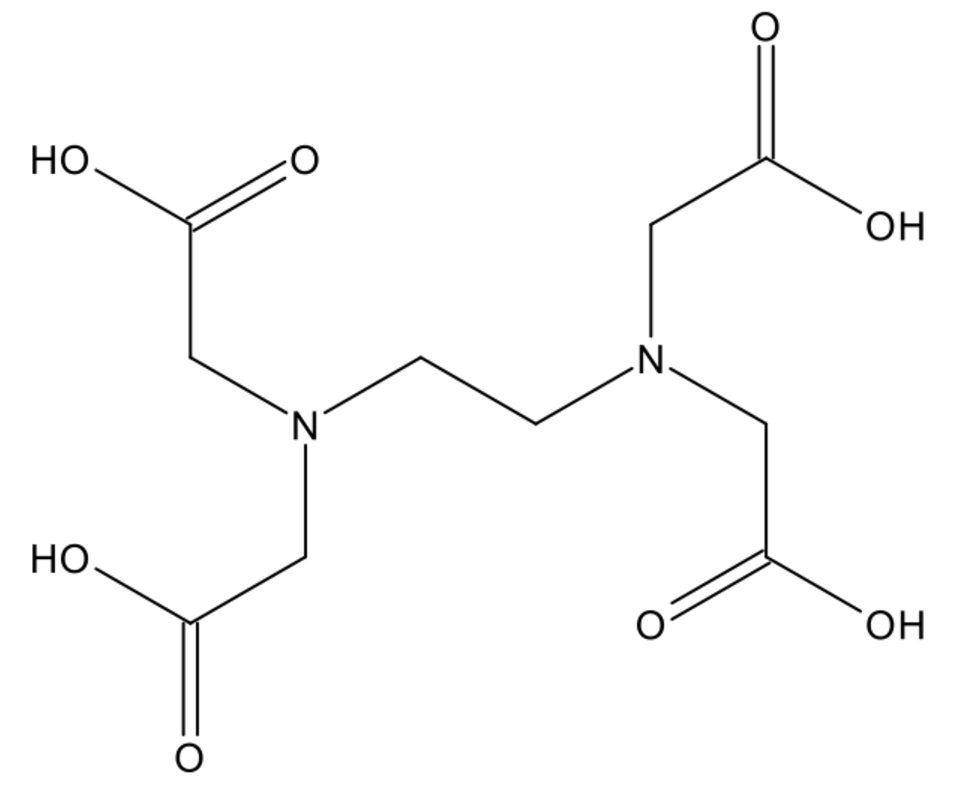
\includegraphics[scale=0.25]{Divers/edta-ro.pdf}
\caption{Molécule d'EDTA}
\end{figure}

Les molécules d'\chemform{EDTA^{2-}} vont se lier avec les ions \chemform{M^{2+}} (exemple Figure \ref{fig:ca-edta}). Un indicateur placé dans l'eau change de couleur quand tout (ou presque) les \chemform{M^{2+}} sont liés avec des molécules d'EDTA, ce qui nous permet de connaître, via le nombre de molécules de d'acide consommé, celui des minéraux (voir Section \ref{sec:pm} et \ref{sec:res}).

\begin{figure}[H]
\centering
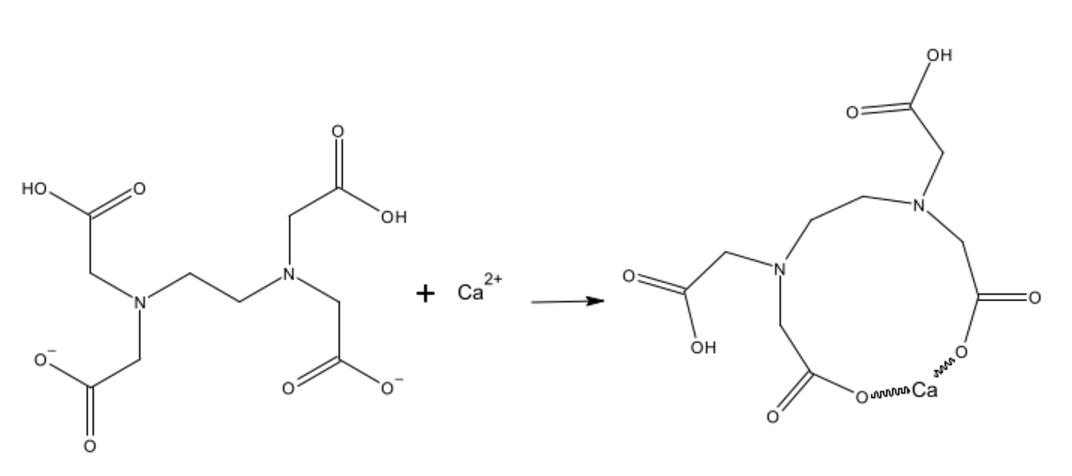
\includegraphics[scale=0.75]{Divers/edta_et_ca-ro.pdf}
\caption{Liaison ionique entre un \chemform{M^{2+}} (dans ce cas \chemform{Ca^{2+}}) et une molécule d'\chemform{EDTA^{2-}}}
\label{fig:ca-edta}
\end{figure}

\section{Principe de mesure et description}
\label{sec:pm}
\subsection{Montage}
\begin{figure}[H]
\centering
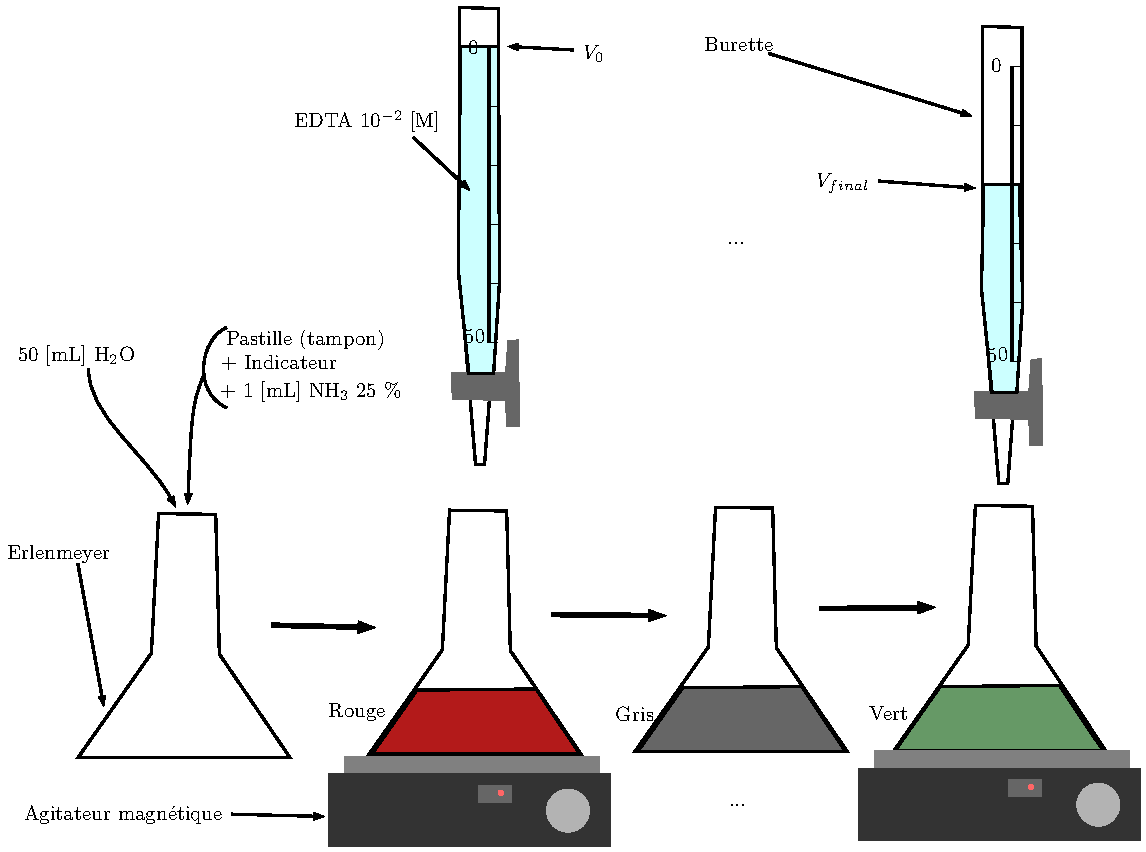
\includegraphics[scale=0.65]{Divers/schema.pdf}
\caption{Schéma du dispositif et du déroulement de l'expérience}
\end{figure}

\subsection{Matériel}
\begin{itemize}
\item 1 Erlenmeyer de 300 [mL] par préparation
\item Éprouvette graduée de 100 [mL]
\item Burette 50 [mL]
\item Agitateur magnétique
\item Solution d'EDTA à $10^{-2}$ M
\item 1 tampon sous forme de pastille par préparation
\item Entonnoir
\item Solution de référence \chemform{NH_3} à 25 \%
\item Bécher
\end{itemize}

\subsection{Mode opératoire}
\begin{enumerate}
    \item Récupérer 50 [mL] d'eau pour chaque échantillon à tester, les transvaser dans un Erlenmeyer, y ajouter quelques gouttes de \chemform{NH_3} puis placer une pastille tampon dans chaque Erlenmeyer.
    \item Remplir la burette d'EDTA quelques centimètre au dessus du 0 avec l'aide de l'entonnoir puis placer le Becher en dessous et vider la Burette jusqu'à ce que le niveau d'EDTA soit au niveau du 0. S'assurer de l'absence de bulle d'air en dessous du robinet sinon recommencer.
    \item Mettre l'aimant dans l'eau et s'assurer que la pastille se soit dissoute, si ce n'est pas le cas, il est possible d'accélérer le processus avec l'agitateur magnétique réglé sur 300 tours minutes.
    \item Une fois la pastille dissoute et l'eau devenue rouge, placer l'Erlenmeyer sous la burette sur l'agitateur magnétique toujours réglé sur 300 tours minutes (réglage à potentiellement modifier dépendant de la taille de l'Erlenmeyer, le but étant que l'eau n'éclabousse pas sur les bords). L'embouchure de la burette doit être placée sous l'entrée du col de l'Erlenmeyer puis on peut faire couler l'EDTA au goutte à goutte dans l'Erlenmeyer.
    \item Observer le contenu de l'Erlenmeyer virer au gris puis au vert. Une fois au vert, arrêter rapidement le goutte à goutte et noter la quantité d'EDTA qui s'est écoulée. On peut faciliter l'observation du changement de couleur en illuminant le mélange avec une lampe.
    \item Recommencer pour chaque échantillon préparer. Entre 2 échantillons, il est possible de remplir ou non la burette à nouveau (si l'on ne remplit pas la mesure précédente devient $V_0$). A noter que ne pas la remplir apporte de l'erreur. De plus, pour avoir une mesure plus précise si le changement de couleur est trop rapide, il est possible de prendre des échantillons de 100 [mL] plutôt que 50.
\end{enumerate}

\section{Résultats}
\label{sec:res}

Connaissant maintenant le volume d'EDTA qu'il faut pour titrer notre eau, il faut aussi trouver les concentrations de \chemform{Ca^{2+}} et \chemform{Mg^{2+}}. La concentration d'EDTA est de $10^{-2} \ [M] = 0,01 [\frac{mol}{L}] $, donc le nombre de mole d'\chemform{H_2 EDTA^{2-}} (pour réagir avec les ions \chemform{M^{2+}}, l'EDTA se sépare de deux \chemform{H^+}) est de $n_{\text{H}_2 EDTA^{2-}} = C_{\text{H}_2 EDTA^{2-}} \cdot V_{\text{H}_2 EDTA^{2-}} = 0,01 \cdot V_{\text{H}_2 EDTA^{2-}} $, avec $V_{\text{H}_2 EDTA^{2-}}$ le volume d'EDTA.\\ \\
Comme dit plus tôt (Section \ref{sec:intro}, Figure \ref{fig:ca-edta}), une mole d'EDTA correspond à une mole de \chemform{M^{2+}}. Connaissant le volume d'eau, il est aisé de connaître la concentration de \chemform{M^{2+}} : $ C_{\text{M}^{2+}} = \frac{n_{\text{M}^{2+}}}{V_{eau}} $ puis de la convertir en degré français $ 1 \ [^\circ f] \sim 0,0001 [M] $ donc $ C_{\text{M}^{2+}} \ [^\circ f] = \frac{C_{\text{M}^{2+}} \ [M]}{0,0001} $. \\ \\
Dans le tableau suivant (Table \ref{tab:mesure}) sont consignées nos mesures. Pour faciliter la lecture, les volumes intermédiaires sont laissés en [mL]. De plus, pour $V_{\text{H}_2 EDTA^{2-}}$, lorsque le référentiel n'est pas à 0, il est noté $V_{final} - V_0 = V_{\text{H}_2 EDTA^{2-}} $.

\begin{table}[H]
\centering
\begin{tabular}{|>{\columncolor{darkgray}}c|c|>{\columncolor{gray}}c|c|>{\columncolor{gray}}c|c|>{\columncolor{gray}}c|}
\hline 
\rowcolor{darkgray} \cellcolor{black} & $V_{\text{H}_2 EDTA^{2-}} \ [mL]$ & $n_{\text{H}_2 EDTA^{2-}} \ [mol]$ & $n_{\text{M}^{2+}} \ [mol]$ & $V_{eau} \ [mL]$ & $C_{\text{M}^{2+}} \ [M]$ & $C_{\text{M}^{2+}} \ [^\circ f]$ \\ 
\hline 
Maison 1-1 & 14,1 & $1,41 \cdot 10^{-4}$ & $1,41 \cdot 10^{-4}$ & 50 & $2,82 \cdot 10^{-3}$ & 28,2 \\ 
\hline 
Maison 1-2 & 28 - 14,1 = 13,9 & $1,39 \cdot 10^{-4}$ & $1,39 \cdot 10^{-4}$ & 50 & $2,78 \cdot 10^{-3}$ & 27,8 \\ 
\hline 
Maison 2 & 39,1 - 28 = 11,1 & $1,11 \cdot 10^{-4}$ & $1,11 \cdot 10^{-4}$ & 50 & $2,22 \cdot 10^{-3}$ & 22,2 \\ 
\hline 
Source & 14,5 - 2 = 12,5 & $1,25 \cdot 10^{-4}$ & $1,25 \cdot 10^{-4}$ & 50 & $2,5 \cdot 10^{-3}$ & 25 \\ 
\hline 
GAP & 21,4 - 14,5 = 6,9 & $6,9 \cdot 10^{-5}$ & $6,9 \cdot 10^{-5}$ & 50 & $1,38 \cdot 10^{-3}$ & 13,8 \\ 
\hline 
\end{tabular}
\caption{Mesure de volume d'EDTA avant changement de couleur et calcul de la dureté de l'eau}
\label{tab:mesure}
\end{table}

Nous n'allons pas faire de tableaux comparatifs avec les valeurs théorique des communes car cela n'est pas du plus pertinent : on trouve des valeurs très différentes selon où l'on recherche.\\
Pour la Maison 1, nous avons mesuré 28,2 et 27,8, soit 28 $[^\circ f]$ de moyenne. Sur le site de la commune de Cossonay\footnote{\href{https://www.cossonay.ch/administration-37/service-des-eaux}{https://www.cossonay.ch/administration-37/service-des-eaux}}, nous apprenons qu'elle devrait avoir une moyenne de 30 degrés français, mais le rapport d'analyse 2021 sur le même site nous indique $26,6 \pm 1,3 \ [^\circ f]$. Dans les deux cas nos mesures sont dans le même ordre de grandeur.\\ \\
C'est plus compliqué pour la Maison 2. Sur le site de la commune de Lutry \footnote{\href{https://www.lutry.ch/vivre-a-lutry/environnement-eau-et-energie/eau/eau-potable/}{https://www.lutry.ch/vivre-a-lutry/environnement-eau-et-energie/eau/eau-potable/}}, nous voyons qu'au Nord de la voix CFF Lausanne-Berne, il est noté 14,8 degrés français, alors que le rapport 2021 (du même site\footnote{\href{https://www.lutry.ch/fileadmin/user\_upload/pdf/SiLy/Lutry\_eau\_qualite\_2021.pdf}{https://www.lutry.ch/fileadmin/user\_upload/pdf/SiLy/Lutry\_eau\_qualite\_2021.pdf}}), annonce 15,1 pour la Croix sur Lutry. Néanmoins on a mesuré 22,2 $[^\circ f]$, ce qui semble une grosse erreur. Cela peut s'expliquer par le fait que les rapports datent d'il y a 2 ans, car on voit dans le même document que l'eau vient de Lausanne, des sources du Pays-d’Enhaut, de la station du lac de Bret et du lac Léman. Or la qualité de l'eau 2022 du site de Lausanne\footnote{\href{https://issuu.com/villedelausanne/docs/eau\_depliant\_2020\_web}{https://issuu.com/villedelausanne/docs/eau\_depliant\_2020\_web}} indique que la dureté de l'eau de ces sources varie entre 13 et 23 $[^\circ f]$, ce qui rendrait notre résultat pertinent.\\ \\
La source privée, d'une fontaine proche de la Maison 2 est estimée à 25 $[^\circ f]$, et n'étant pas du réseau communal on n'a pas de valeur de référence. Finalement, celle du gymnase Auguste Piccard (GAP) est mesurée à 13,8 et le site de la commune de Lausanne\footnote{\href{https://www.lausanne.ch/vie-pratique/energies-et-eau/eau/qualite/reservoir-recherche/reservoir-resultat?adresse=chemin\%20de\%20Bellerive\%2016\%20LAUSANNE}{https://www.lausanne.ch/vie-pratique/energies-et-eau/eau/qualite/reservoir-recherche/reservoir-resultat?adresse=chemin\%20de\%20Bellerive\%2016\%20LAUSANNE}} indique une dureté moyenne de 14 $[^\circ f]$, donc la mesure est très bonne. \\
Finalement, le tableau ci-dessous (Table \ref{tab:durete}) montre la dénomination courante de nos différentes mesures.

\begin{table}[H]
\centering
\begin{tabular}{p{0.05\textwidth}l|l|c|}
\cellcolor{cyan} & Douce & Inférieure à 15 $[^\circ f]$ & GAP \\ 
\cellcolor{blue} & Moyenne & De 15 $[^\circ f]$ à 25 $[^\circ f]$ & Maison 2 \\ 
\cellcolor{yellow} & Assez dure & De 25 $[^\circ f]$ à 32 $[^\circ f]$ & Maison 1, Source \\ 
\cellcolor{pink} & Dure & De 32 $[^\circ f]$ à 42 $[^\circ f]$ &  \\ 
\cellcolor{red} & Très dure & Supérieure à 42 $[^\circ f]$ &  \\ 
\end{tabular} 
\caption{Dureté selon le degré français de l'eau}
\label{tab:durete}
\end{table}

\section{Discussion}

Les résultats obtenus sont globalement très similaires à ceux officiels. Cela est très satisfaisant, et montre qu'un dispositif assez "simple" permet de réaliser de telles mesures.\\ \\
On peut malgré tout noter quelques sources d'erreurs. Tout d'abord celles basiques liées à l'observateur : mesure du volume d'EDTA et d'eau principalement, ainsi que peut être la concentration de l'EDTA qui n'est pas exacte. \\
Il y a aussi celles spécifiques au titrage complexiométrique et à notre montage : la nécessité de faire à l’œil pour repérer le changement de couleur de notre échantillon, la précision de la burette si on doit redémarrer la mesure (si l'échantillon est gris et ne passe pas au vert), et finalement le dosage des différent réactif qui sont liés au protocole mais dont on ne nous indique pas les rôles exactes et l'impact qu'ils ont.\\
De plus, le transport de l'eau depuis les maisons se sont faits dans des gourdes, considérées propres mais il n'est pas à omettre des traces de minéraux mal nettoyés, ou au contraire ceux des échantillons auraient pu s'y déposer et donc légèrement modifier les mesures. \\ \\
Ensuite il est intéressant de remarquer les duretés selon la localisation géographique. On remarque que le GAP, qui a de l'eau du lac, à une eau dite douce, donc avec une faible concentration en minéraux. En revanche, celle de Cossonay venant des roches du Jura est assez dure, et il y a le même constat pour la source. Ces deux constatations laissent à penser que l'eau de la Maison 2 doit venir en cette saison des sources du Pays-d’Enhaut, car elle est de dureté moyenne, plutôt haute, et l'on voit que les lacs ont tendance à être dans douce ou moyenne plutôt basse.

\section{Conclusion}

En conclusion, nous sommes satisfaits de ce que nous avons obtenu. Ils sont d'une précision remarquable vis à vis de la simplicité du montage. Il y a quand même des voies d’améliorations de l'expérience. On pourrait utiliser de plus grande quantité d'eau et faire la mesure sur une plus grande durée afin d'être plus précis. Il serait aussi envisageable de doubler avec d'autre principe de mesure, par exemple réussir à récupérer le \chemform{M^{2+}} par un principe physique (laisser l'eau évaporer, les forcer à s'agglutiner sur les parois ou autre). Une modification pertinente de l'expérience serait de trouver des substances permettant de coloré l'eau selon des intervalles de dureté (comme par exemple dans la Table \ref{tab:durete}). Finalement il est bien de noter que les résultats obtenus mettent bien en évidence le lien entre le trajet à travers le sol et sa dureté.

\end{document}